\part{Flowcharts}
\frame{\partpage}

\begin{frame}
	\begin{center}
		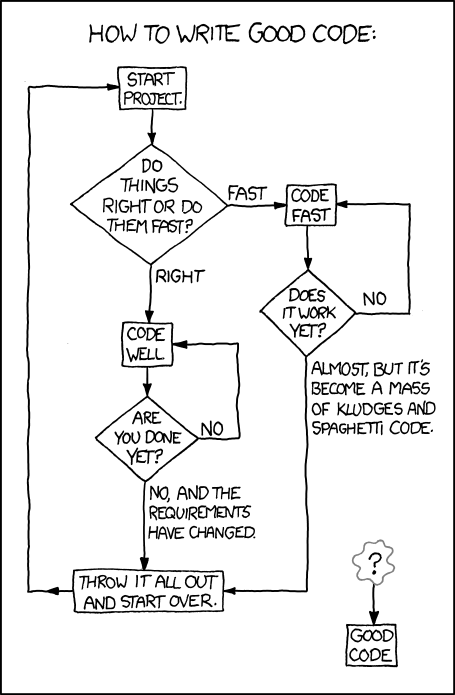
\includegraphics[height=0.9\textheight]{xkcd_good_code}
		
		{\tiny\url{http://xkcd.com/844/}}
	\end{center}
\end{frame}

\begin{frame}{Flowchart symbols}
	\begin{center}
		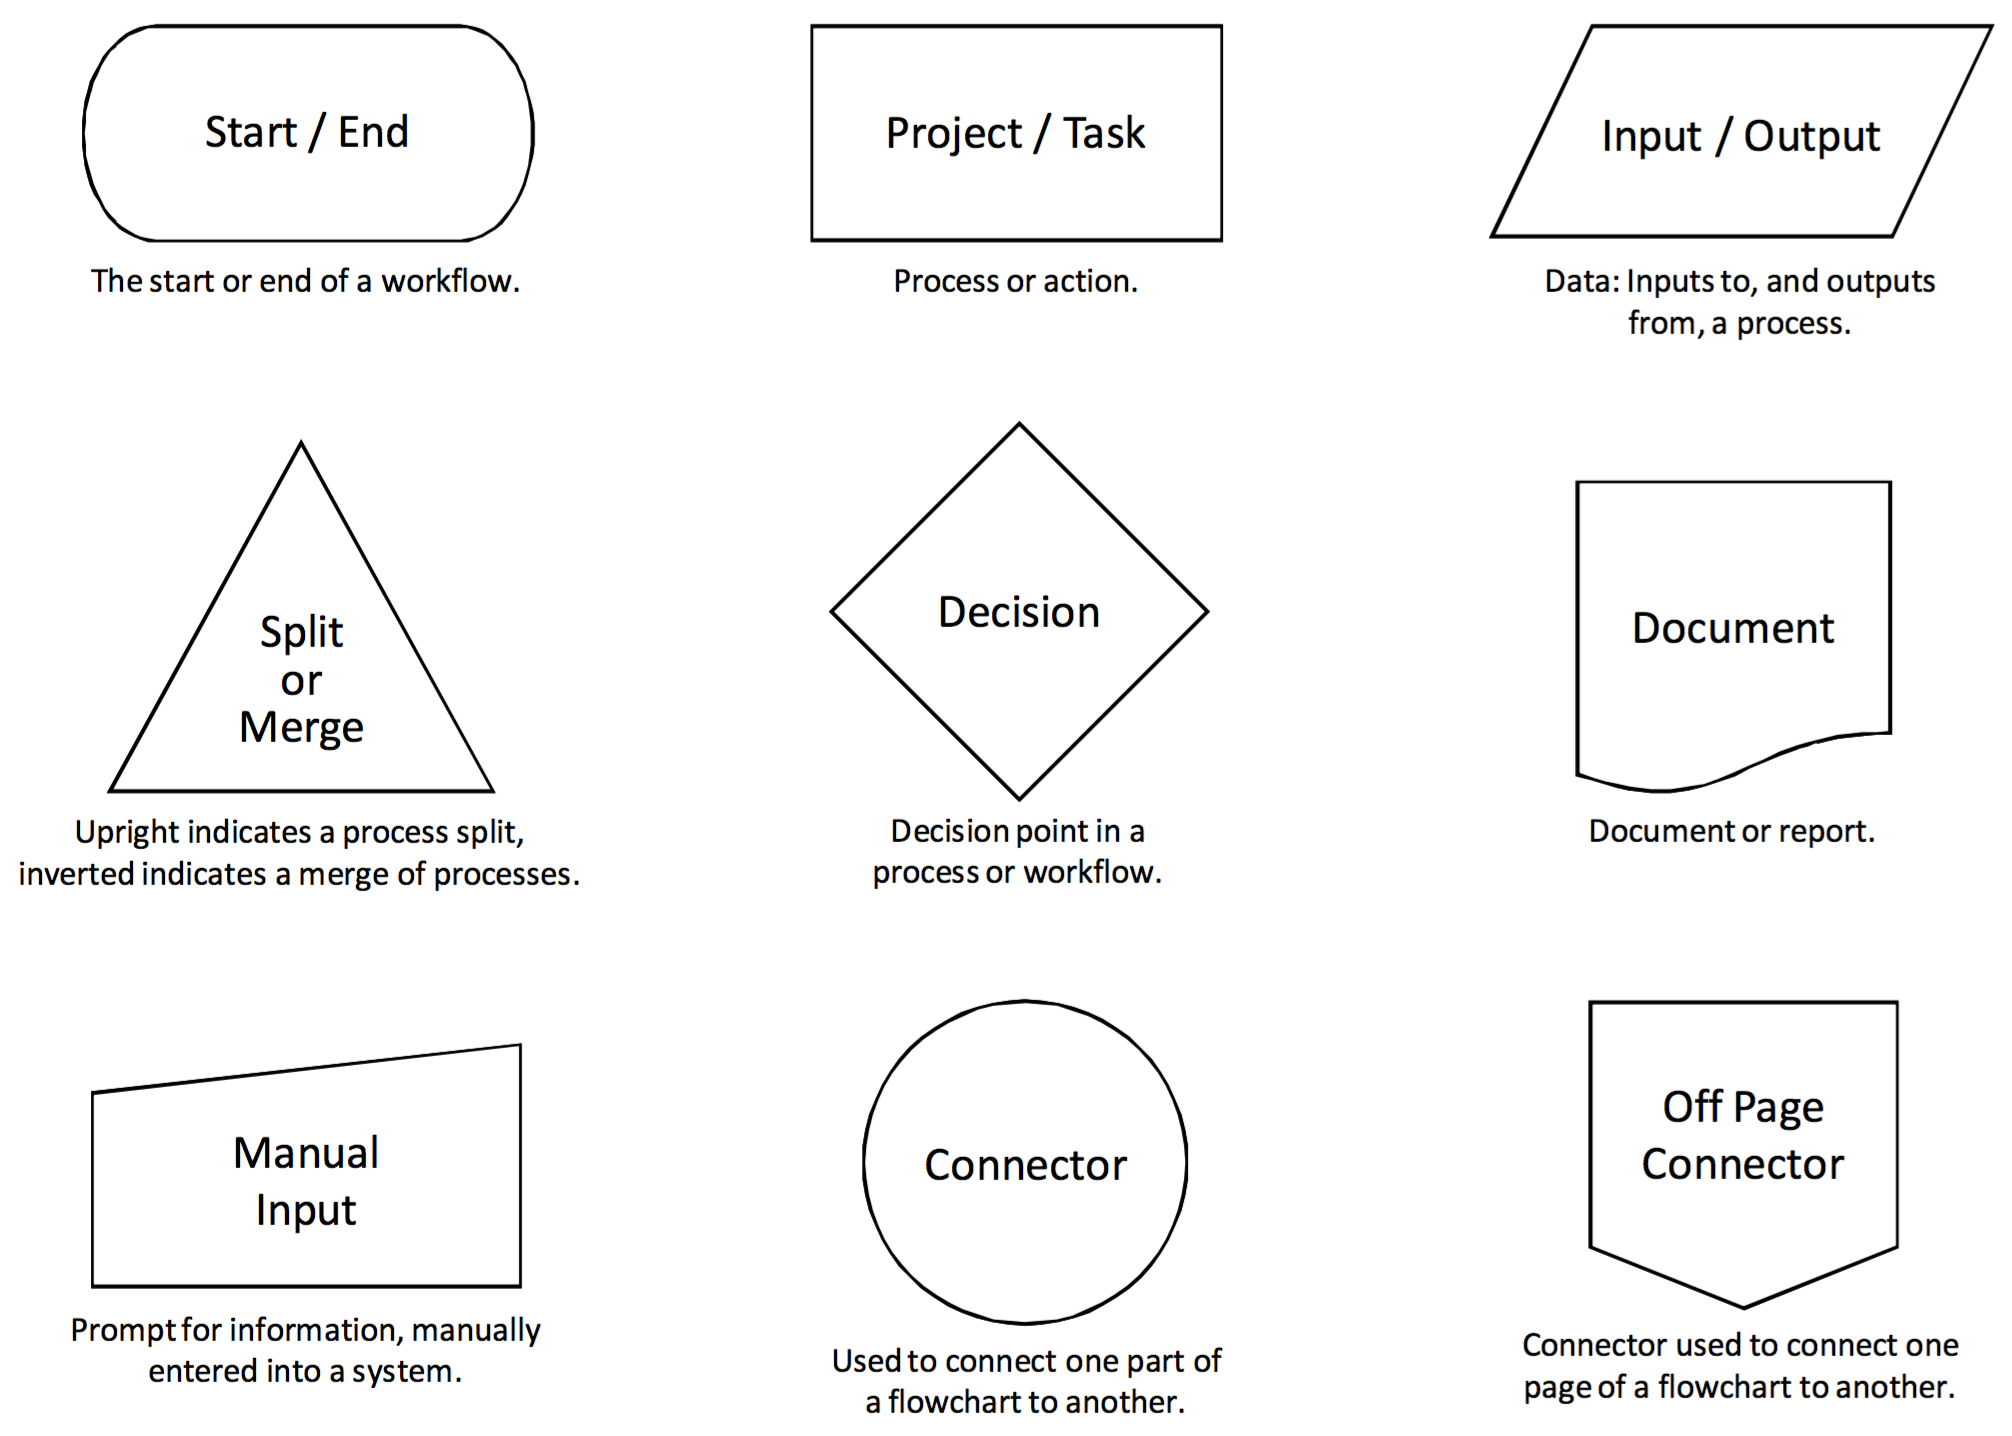
\includegraphics[height=0.8\textheight]{flowchart_symbols}
	\end{center}
\end{frame}

\begin{frame}{Swimlanes}
	\begin{center}
		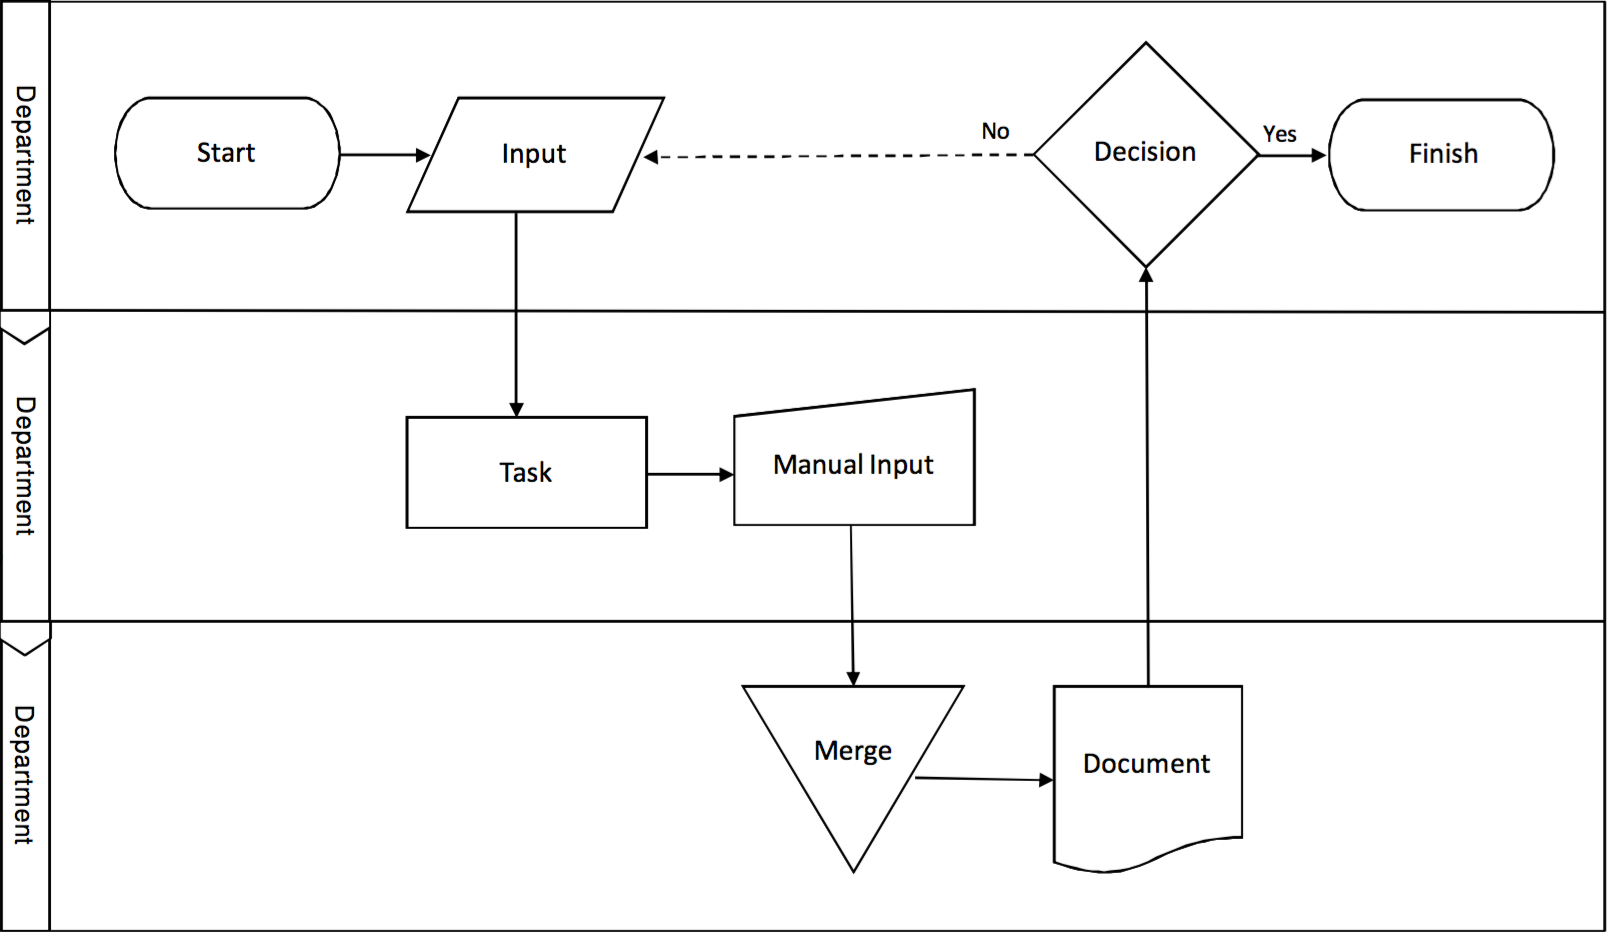
\includegraphics[width=\textwidth]{swimlanes}
	\end{center}
\end{frame}

\begin{frame}{Software for drawing flowcharts}
	\pause Intended for drawing flowcharts:
	\begin{itemize}
		\item Gliffy \url{https://www.gliffy.com}
		\item LucidChart
		\item Microsoft Visio
	\end{itemize}
	\pause Can draw flowcharts:
	\begin{itemize}
		\item Microsoft PowerPoint
		\item Google Docs
	\end{itemize}
	\pause If you're desperate:
	\begin{itemize}
		\item Any drawing package (Inkscape, Adobe Illustrator, Apple Keynote, ...)
		\item MS Paint
		\item Pen and paper
	\end{itemize}
\end{frame}

\begin{frame}{Activity}
	\begin{itemize}
		\item In \textbf{groups of 2-3}
		\item \textbf{Draw} a flowchart for \textbf{logging into Facebook}
		\item Include at least two swimlanes: \textbf{the user's browser/device} and \textbf{the Facebook server}
		\item Post your flowchart to \textbf{\#comp110 on \url{https://falmouthgamesacademy.slack.com}}
	\end{itemize}
\end{frame}

\begin{frame}{UML activity diagrams}
	\begin{itemize}
		\pause\item Modern counterpart of flowcharts
		\pause\item UML = Unified Modeling Language --- defines 14 types of diagram to represent various aspects of computing systems, of which activity diagrams are one
	\end{itemize}
	\pause
	\begin{center}
		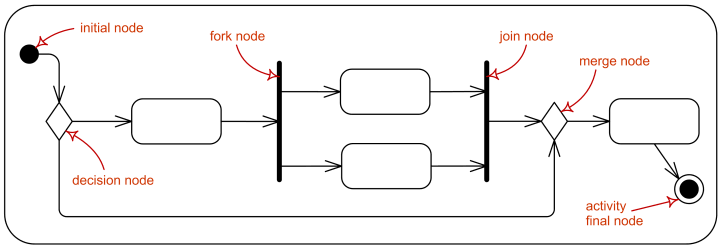
\includegraphics[width=0.9\textwidth]{uml_symbols}
	\end{center}
\end{frame}

